\documentclass[journal,12pt,twocolumn]{IEEEtran}
\usepackage{amsmath,amssymb,amsfonts,amsthm}
\usepackage{txfonts}
\usepackage{tkz-euclide}
\usepackage{listings}
\usepackage{gvv}
\usepackage[latin1]{inputenc}
\usepackage{array}
\usepackage{pgf}
\usepackage{lmodern}

\begin{document}
\bibliographystyle{IEEEtran}

\vspace{3cm}

\title{}
\author{EE23BTECH11024 - G.Karthik Yadav$^{*}$
}
\maketitle
\newpage
\bigskip

\section*{GATE 2023 EC 41}
\noindent 1. \hspace{2pt} A Closed loop systen is shown in the figure where $k>0$ and $\alpha>0$ .\\
The Steady State error due to a ramp input $\brak{R\brak{s} = \alpha s^{-2}}$ is given by \hfill{(GATE 2023 EC 41)}

\begin{figure}[ht]
\centering
    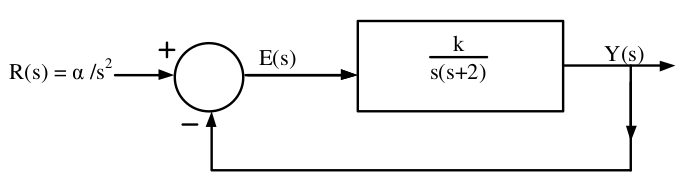
\includegraphics[width=1.0\linewidth]{figs/question.png}
    \label{fig: 23.EC.41.24.1}
\end{figure}

\begin{enumerate}
\item $\frac{2\alpha}{k}$
\item $\frac{\alpha}{k}$
\item $\frac{\alpha}{2k}$
\item $\frac{\alpha}{4k}$
\end{enumerate}

\solution

\setlength{\arrayrulewidth}{0.2mm}
\setlength{\tabcolsep}{15pt}
\renewcommand{\arraystretch}{1.3}


\begin{table}[ht]
  \centering
  \begin{tabular}{|c|c|c|}
    \hline
    	Symbol & Parameters & value\\
    \hline
	  $R\brak{s}$ & Ramp input signal  &  $\alpha s^{-2}$\\
    \hline
	  $G\brak{s}$ & Open Loop transfer function &  $\frac{k}{s\brak{s+2}}$\\
    \hline
         $e_s$ & Steady State Error &  ? \\
    \hline
         $K_v$ & velocity constant &  ? \\
    \hline
  \end{tabular}
  \vspace{0.3cm}
  \caption{Input Parameters}
  \label{tab:2023.EC.41.T1}
\end{table}


from table \ref{tab:2023.EC.41.T1}
,,Open loop transfer function $G\brak{s}$\\
\begin{align}
	G\brak{s} &= \frac{Y\brak{s}}{E\brak{s}} \label{24.2023.EC.41.1} \\
        &= \frac{Y\brak{s}}{R\brak{s} - Y\brak{s}} \\
        Y\brak{s} &= \frac{R\brak{s}G\brak{s}}{1 + G\brak{s}} \label{24.2023.EC.41.2}
\end{align}

from eq \eqref{24.2023.EC.41.1} and eq \eqref{24.2023.EC.41.2}

\begin{align}
        G\brak{s} &= \frac{k}{s\brak{s +2}}  \label{24.2023.EC.41.3} \\ 
        Y\brak{s} &= \frac{\alpha k s^{-2}}{k + s\brak{s+2}} \label{24.2023.EC.41.4} \\
        E\brak{s} &= R\brak{s} - Y\brak{s}  \label{24.2023.EC.41.5} \\ 
        E\brak{s} &= \frac{R\brak{s}}{1 + G\brak{s}}
\end{align}

By Taking Inverse Laplace Transform of eq \eqref{24.2023.EC.41.3} and eq \eqref{24.2023.EC.41.4}

\begin{align}
	g\brak{t} &= \frac{k\brak{1 - e^{-2t}}}{2} u\brak{t}
\end{align}

\begin{align}
    e_s &= \displaystyle\lim_{s\to 0}s E\brak{s} \\
    &= \displaystyle\lim_{s\to 0} s \frac{R\brak{s}}{1 + G\brak{s}} \\
    &= \displaystyle\lim_{s\to 0} \frac{\alpha \brak{s+2}}{s\brak{s+2} + k} \\
    e_s &= \frac{2\alpha}{k}
\end{align}
\\
\\
\begin{figure}[ht]
\centering
    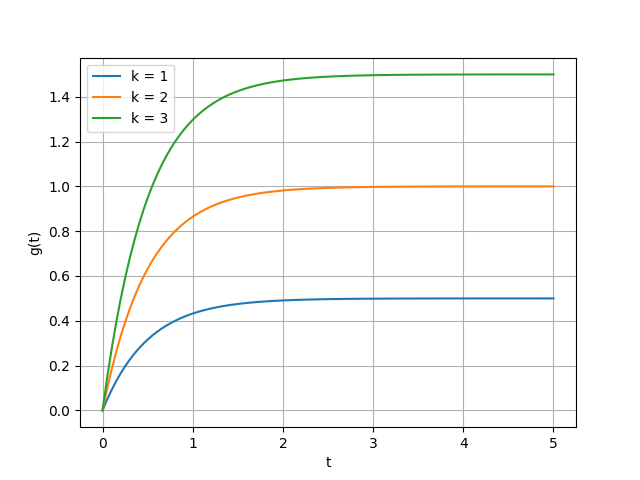
\includegraphics[width=0.95\linewidth]{figs/gate.png}
    \label{fig: 23.EC.41.24.2}
    \caption{Plot of $g\brak{t}$ vs t }
\end{figure}


\end{document}
